Neste capítulo serão apresentadas as funcionalidades disponíveis aos usuários finais do sistema.
 É possível emitir, visualizar, exportar e revogar um certificado digital, bem como acessar as páginas de ajuda e de repositório do sistema.

\section{Emissão de Certificado}

No menu \textit{Certificado} é possível encontrar as ações de emitir e revogar, como mostra a figura \ref{fig:emirevog}:

\begin{figure}[ht]
     \centering
     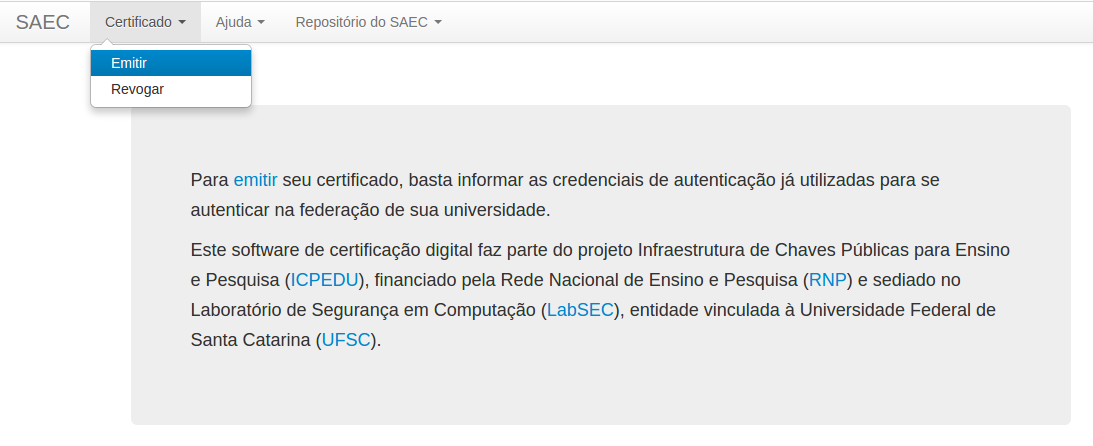
\includegraphics[scale=0.4]{images/emitir1.png}
     \caption{Tela inicial}
     \label{fig:emirevog}
\end{figure}

Para emitir, é necessário selecionar a instituição na qual você é afiliado. Seguiremos o manual utilizando a Universidade Federal de Santa Catarina (UFSC) como exemplo de instituição provedora de identidade. Ao ser redirecionado para a tela de escolha de Federação, selecione sua instituição. Você será redirecionado para a página de autenticação da sua instituição, onde deve entrar com os dados do seu usuário já cadastrado. Os passos descritos aqui podem ser observados nas figuras \ref{fig:ufxc} e \ref{fig:ufxc2}.

\begin{figure}[ht]
     \centering
     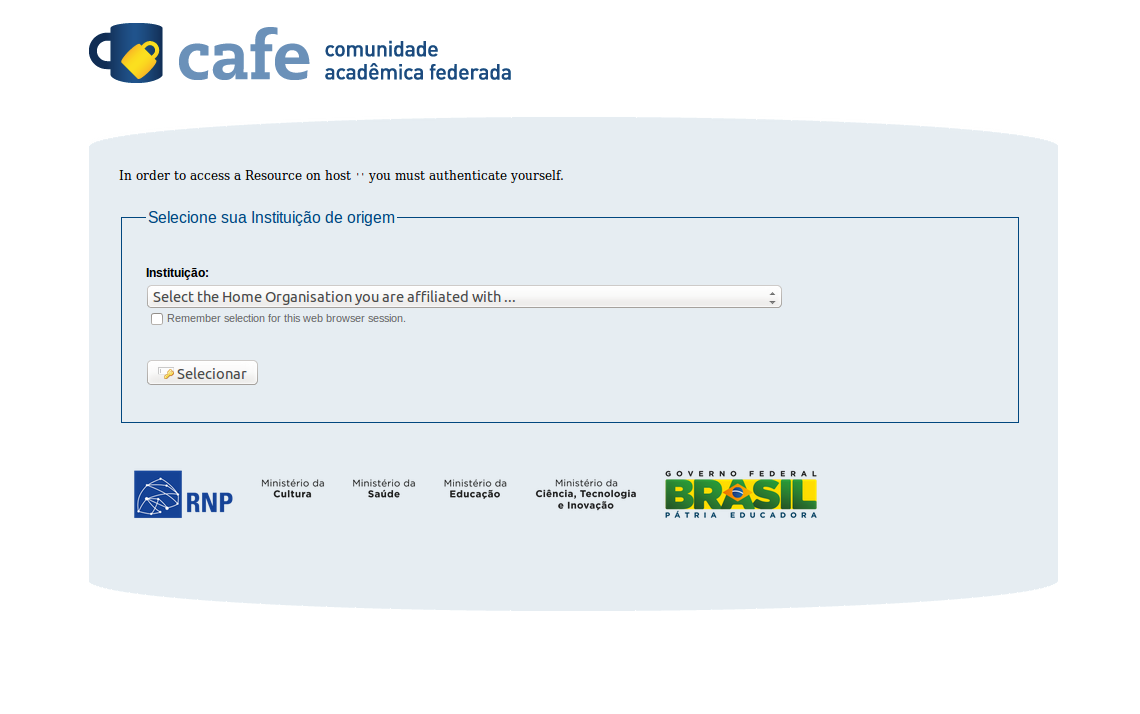
\includegraphics[scale=0.3]{images/escolher-federacao.png}
     \caption{Escolha de Federação}
     \label{fig:ufxc}
\end{figure}

\begin{figure}[ht]
     \centering
     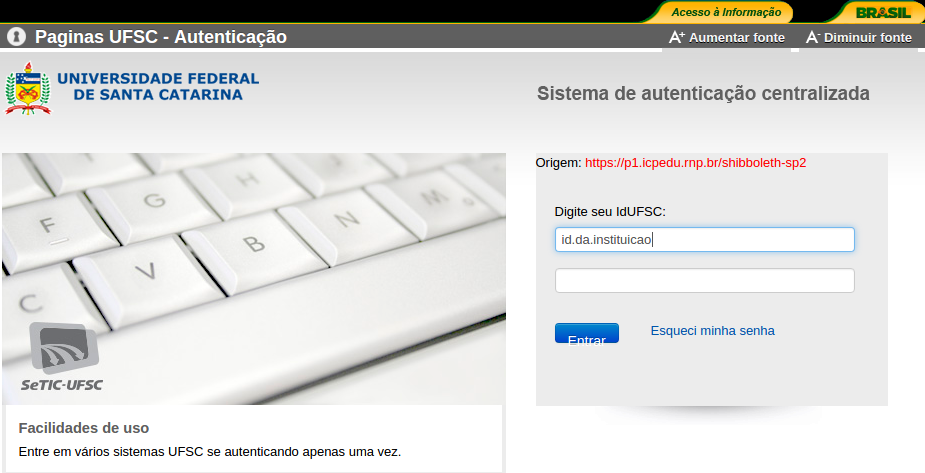
\includegraphics[scale=0.3]{images/emitir2.png}
     \caption{Autenticação na Federação}
     \label{fig:ufxc2}
\end{figure}

Se você já possui um certificado emitido nesta Autoridade Certificadora, e este ainda estiver ativo, um erro aparecerá na tela solicitando que o usuário confirme a emissão de um novo certificado digital, ou cancele a solicitação do mesmo.

Confirme que você deseja emitir um novo certificado em seu nome. A partir desta confirmação, o usuário verá uma tela com seus dados (Nome, CPF, E-mail e Data de  nascimento), onde nenhum deles pode ser editado. Basta conferir os dados e submeter a solicitação de certificado. Vide figura \ref{fig:emissao3}.

Quando o certificado for emitido, no canto superior esquerdo da tela aparecerá uma opção para visualizar o certificado (suas informações, detalhes e OIDs). Ao visualizar o certifica digital emitido, é possível conferir os dados gerais do certificado, em sua aba principal (imagem \ref{fig:geralcert}), e os detalhes do mesmo, em sua aba \textit{Details} (imagem \ref{fig:detailscert}).

\begin{figure}[ht]
     \centering
     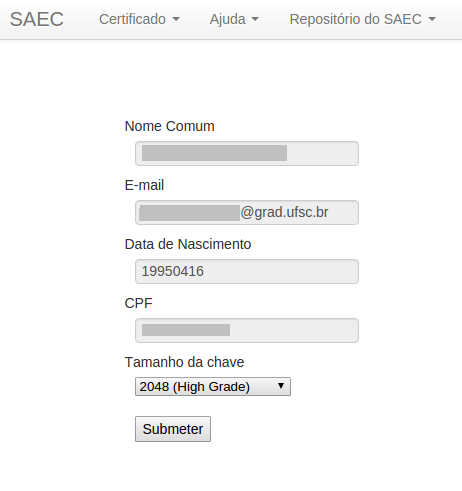
\includegraphics[scale=0.5]{images/emitir3.png}
     \caption{Confirmação de dados}
     \label{fig:emissao3}
\end{figure}

\begin{figure}[ht]
     \centering
     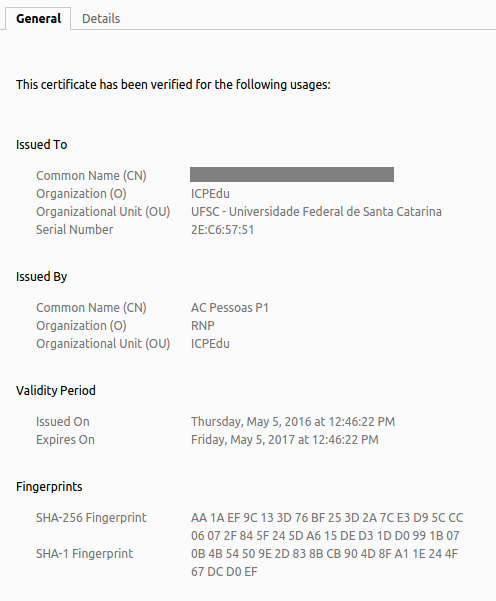
\includegraphics[scale=0.5]{images/geralcert.png}
     \caption{Informações gerais do certificado}
     \label{fig:geralcert}
\end{figure}

\begin{figure}[ht]
     \centering
     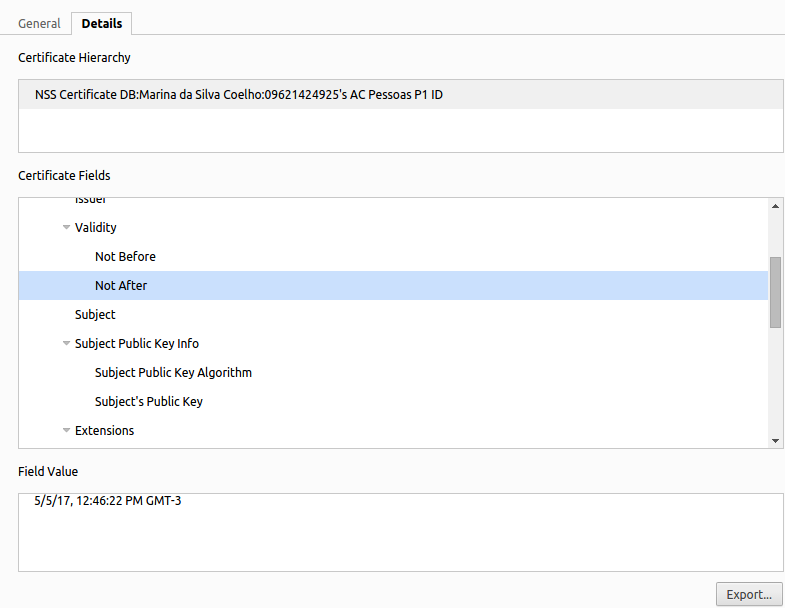
\includegraphics[scale=0.5]{images/details.png}
     \caption{Detalhes do certificado}
     \label{fig:detailscert}
\end{figure}

Como é possível ver na imagem \ref{fig:detailscert}, no canto inferior direito da tela de visualização de certificado, pode-se exportar o mesmo. A etapa para exportar o certificado envolve gerenciamento da chave do mesmo. Como este tipo de configuração é diferente para cada navegador (que também operam de maneira diferente dependendo do sistema operacional da máquina), o usuário deve se dirigir ao menu de ajuda, especificado na seção 7.2, onde poderá encontrar um guia detalhado de como exportar o certificado com base no navegador e sistema operacional utilizados no momento da exportação.

\section{Ajuda}

No menu \textit{Ajuda} é possível encontrar um guia que demonstra o passo a passo para todas as atividades do sistema, desde emissão do seu próprio certificado digital, até a configuração do cliente de e-mail. Basta clicar no menu e seguir as dicas da página.

\section{Repositório}

No menu \textit{Repositório do SAEC} é possível encontrar o certificado da Autoridade Certificadora, que será automaticamente instalado no caso de o usuário utilizar o navegador Mozilla Firefox, ou precisa ser manualmente instalado, caso o usuário use Google Chrome, Internet Explorer ou Safari. Para acessar o guia de instalação, basta clicar no link \textit{Ajuda com a instalação}, posicionado ao lado do certificado a ser baixado.

É possível também baixar a Lista de Certificados Revogados (LCR) da AC. Para instalar a LCR, é necessário, novamente, clicar no link \textit{Ajuda com a instalação}, disponibilizado ao lado da LCR. Ambos os links de ajuda redirecionarão o usuário para a página de ajuda, apresentada na seção 7.2.

